\chapter{AL-IS railways}

\resp{Vicentini Gioele}

\emph{
Structure as\footnote{Remove this part from the report}:
\begin{itemize}
\item A short (max 1 page) explanation of the task, including references. Include mathematical concepts.
\item Max 2 pages for the whole task (including figures)
\item It is possible to use appendices for supplementary material, at the end of the report. Max 5 pages per task
\end{itemize}
A total of 3 pages + 5 supplementary pages per task
}

\section{Introduction: Structure of the dataset}
The dataset contains both the aggregated data for the whole European union (states from AL to IS) and data for each single state. 

The needed data is contained in the shapefile of a chosen directory. 
Each directory contains two specific files:
\begin{itemize}
    \item \texttt{RailrdC.shp}, containin informations about train stations and in particular the needed \texttt{ID}, \texttt{RStationID}, the original name (transliterated, so the field \texttt{NAMA1}), geographic coordinates, the international code of the country (\texttt{ICC}) and its name.
    \item \texttt{RailrdL.shp}, containing the individual pieces of the railway. From this file it's only needed the startpoints and endpoints of the elements. This is because as pointed out in the guide to the user of the dataset, by standard the individual pieces cannot overlap with stations if not at their endpoints.
\end{itemize}
Since the entry \texttt{RStationID} is actually repeated across different nodes, the ID of the stations had to be created ad hoc procedurally and as such station ID's may change in between the single state file and the aggregated data file.

\section{The dataset in numbers, Denmark versus Germany}
Denmark's railway network is relatively small ($\sim 10^2$ stations) when compared with the train infrastructure of Germany or France ($\sim 10^3$). This implies that different kinds of topologies were implemented to both cover a greater (and morphologically different) geographical area and contain the train traffic which consequently emerges. In numbers, this can be seen in \autoref{fig:Deg_dist}: while in Denmark the highest frequency is associated with stations connected to only two other stations, in a "linear" fashion, in Germany both $3$ and $4$ connections are present, as the infrastructure has multiple bifurcations which raise the right side of the curve.

\begin{figure}
    \includegraphics[width=0.45\linewidth]{images/Deg_DE.png}
    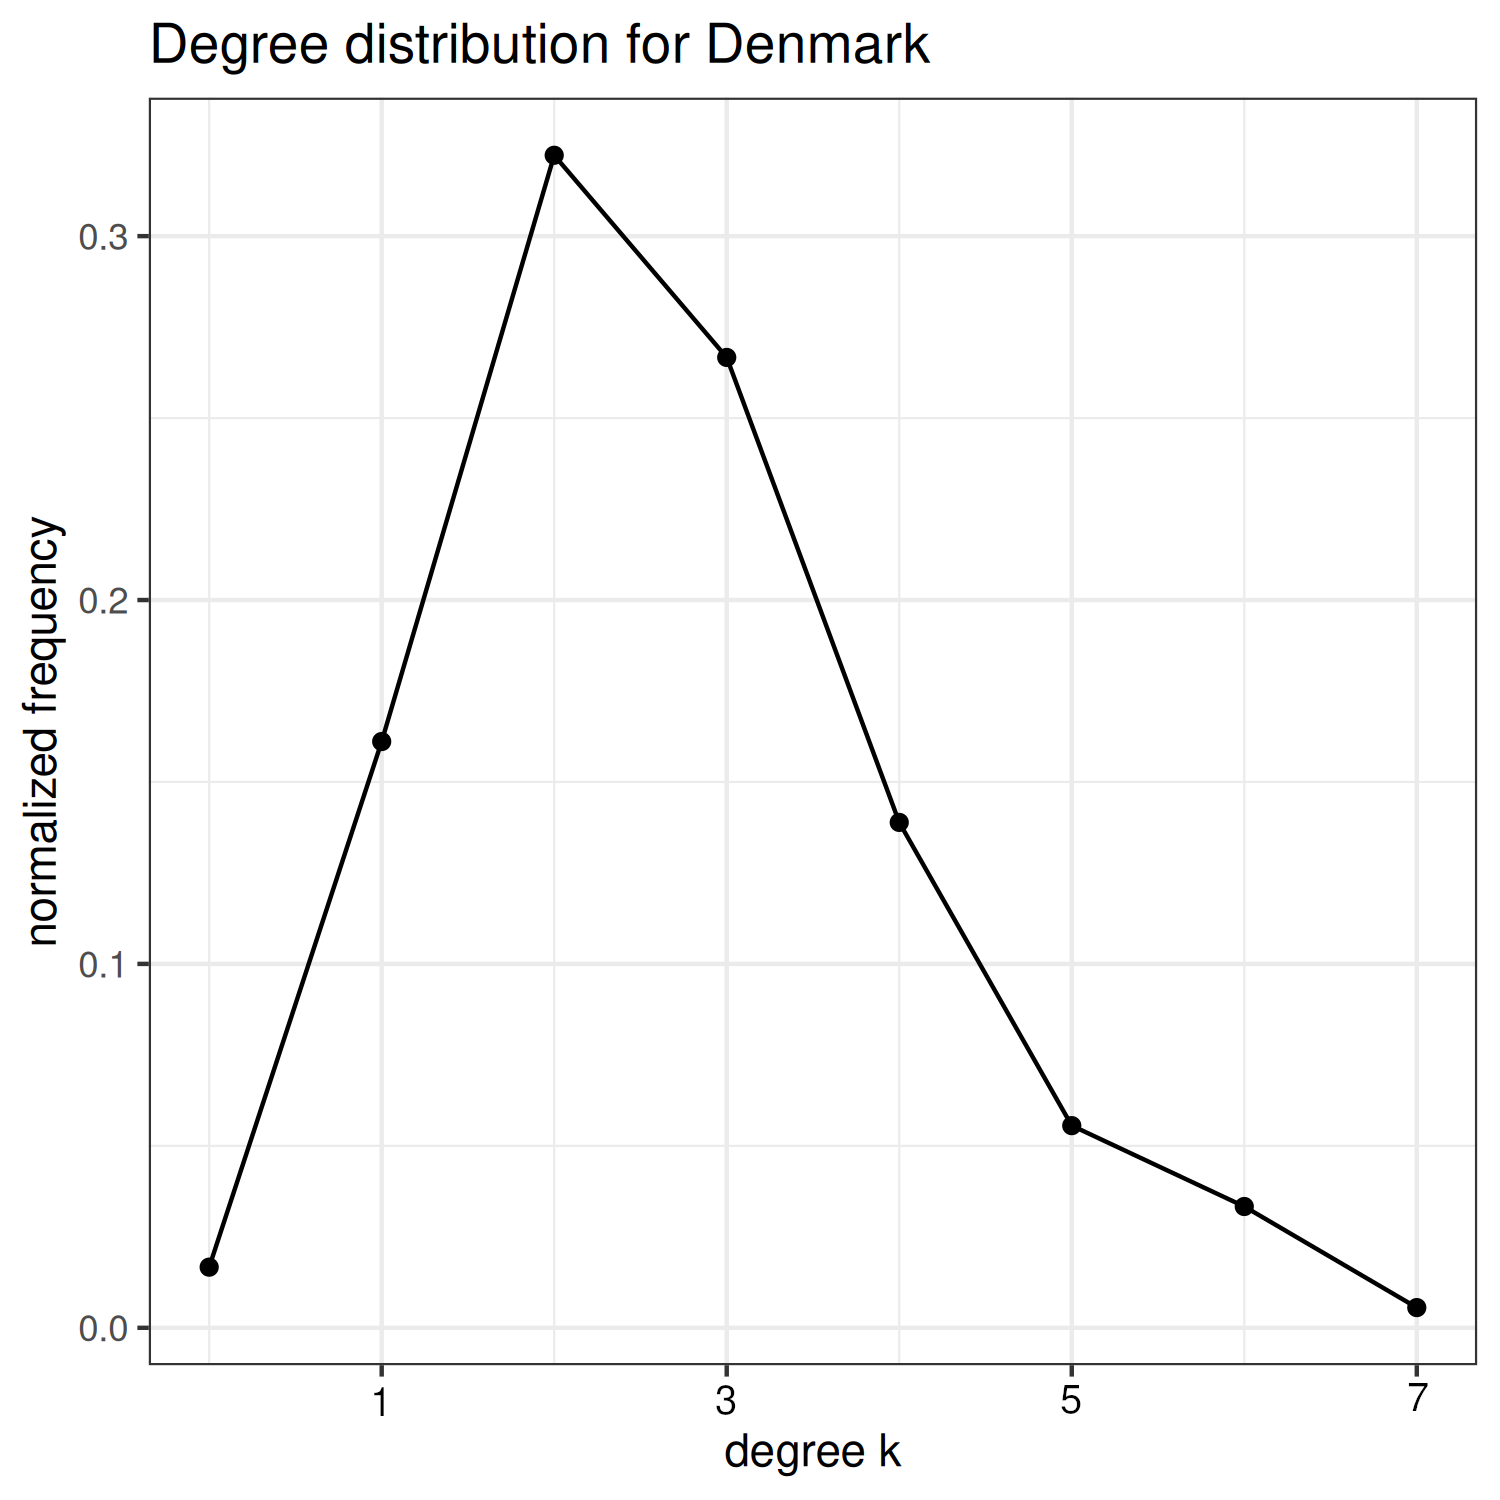
\includegraphics[width=0.45\linewidth]{images/Deg_DK.png}
    \label{fig:Deg_dist}
    \caption[short]{Degree distributions for the railways of Germany (left) and Denmark (right). Different topologies impact the shape of the curve.}
\end{figure}
